\section{The Cicada Framework}\label{sec:cicada_framework}

We present Cicada, our framework for non-interactive private auctions/elections, in \Cref{fig:cicada}. Cicada can be applied to voting and auction schemes where the scoring function $\Score = f \circ t$ has a linear tally function $t$. The framework uses a linear HTLP (\Cref{sec:tlp}), a vector packing scheme (\Cref{sec:packing}), and matching NIZKs (which we present in \Cref{sec:sigmas}) to ensure correctness of submissions by proving both the well-formedness of the puzzle and the solution's membership in $\X$.

% \subsection{System Model}\label{sec:cicada_model}

\begin{figure}[tb]
    \centering
    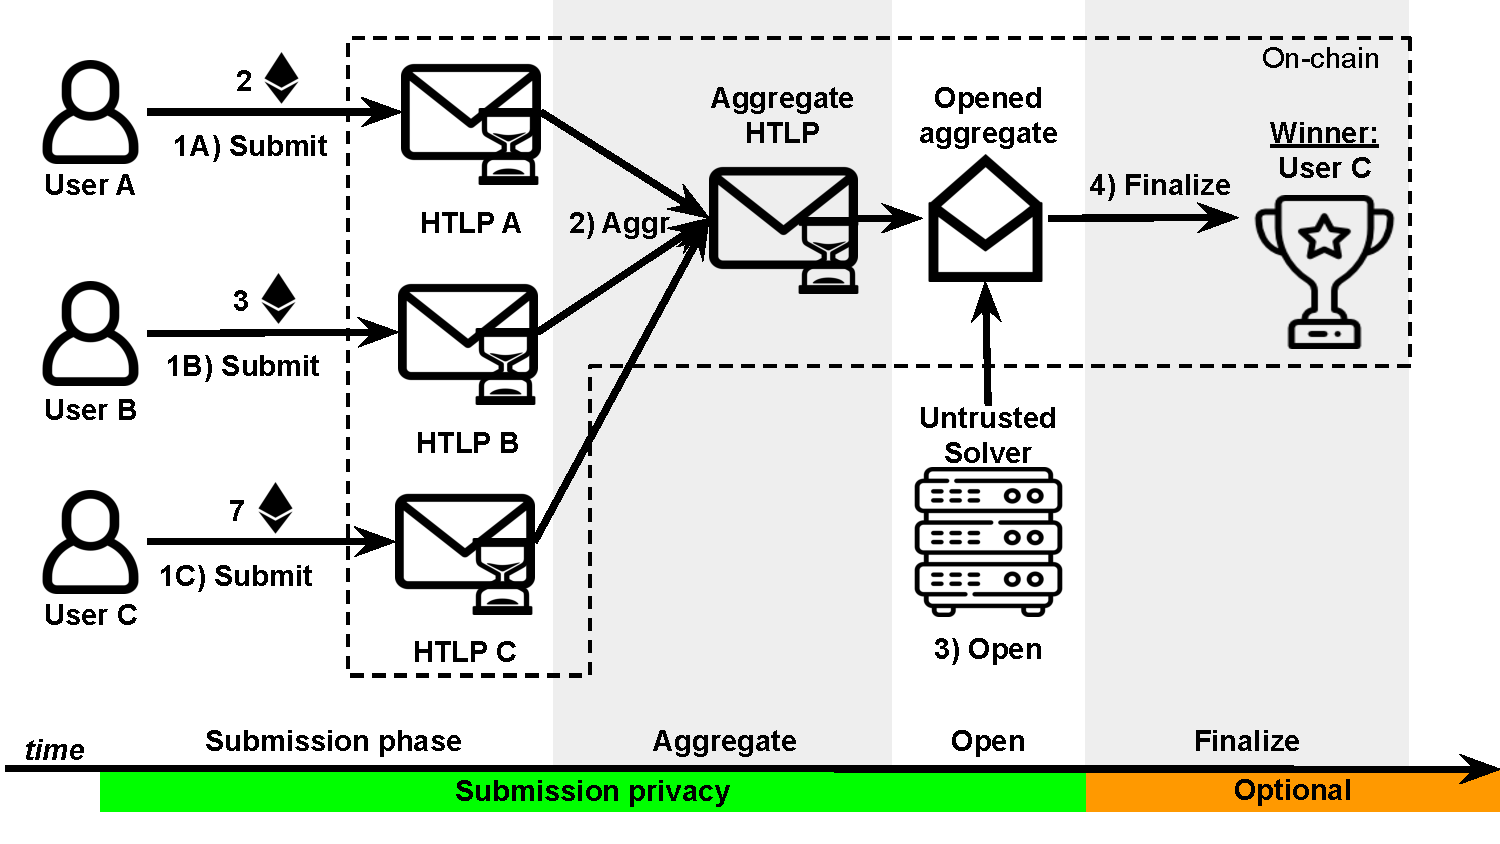
\includegraphics[width=0.95\textwidth]{cicada/figs/cicada-explainer.pdf}
    \caption{The system model of Cicada. \emph{(1) Submission phase:} users generate their bids/ballots as HTLPs and post them to a public bulletin board, e.g., a blockchain. \emph{(2) Aggregation:} an on-chain contract homomorphically combines submissions into an aggregate puzzle as they are submitted. \emph{(3) Opening:} after all submissions have been aggregated, an off-chain entity solves the aggregate HTLP using $\Ttime$ sequential steps and submits the solution to the contract. \emph{(4) Finalize:} The smart contract may do some final computation over the solution to compute the result and announces the winner. Submission privacy is ensured only until the start of the $\mathsf{Open}$ phase. 
    In \Cref{sec:everlasting_ballot_privacy}, we show how voters can pool their submissions to achieve everlasting ballot privacy.
    }
    \label{fig:cicada-explainer}
\end{figure}


We envision three types of participants, as illustrated in \Cref{fig:cicada-explainer}:
\begin{description}
    \item[Users.] We simply refer to voters or bidders as \emph{users}. Users submit bids or ballots, which we generically call \emph{submissions}. We assume some external process to establish the set of authorized users (which may be open to all).  Once users place their submissions, no further action is required of them. 
    \item[On-chain coordinator.] We refer to the tallier/auctioneer as the \emph{coordinator}, typically implemented as a smart contract that collects submissions. The coordinator transparently calculates the winner(s). In the case of an auction, they might also transfer (digital) assets to the winner(s). In an election, they might grant special privileges to the winner.%'s public key.
    \item[Off-chain solver.] We assume an untrusted \emph{solver} who unlocks the final (set of) HTLP off-chain and submits the solution(s) to the coordinator with a proof of correct opening. In principle, this could be any party, but in practice will likely be one of the parties participating in (or administering) the vote/auction or a paid marketplace~\cite{EPRINT:Abadi23,CCS:TGBKS21}.
\end{description}

Cicada implements a time-locked auction/voting scheme (\Cref{def:syntax}) as follows:
(0) System participants agree on a delay parameter $\Ttime$ and packing parameter $\ell$. The latter introduces a crucial design choice, defining a storage-computation trade-off we detail in~\Cref{sec:cicada_eval}. The coordinator (or a set of trusted parties, depending on the HTLP construction used) runs the $\Setup$ algorithm to output HTLP public parameters $\pparam$ and initialize a (set of) aggregate HTLP(s) $\Z$ containing zeros. 
(1) A user $i$ runs the $\Seal$ algorithm to encode their submission (a bid or ballot) $\vec{v}_i$ into (a set of) HTLP(s) $\Z_i$. $\Seal$ also outputs a NIZK $\pi_i$ proving that $\Z_i$ is well-formed, i.e., its contents are in the domain $\X$ of the scoring function $\Score$. Users send their submissions and proofs to the on-chain coordinator. 
(2) Upon receiving a user submission $\Z_i, \pi_i$, the coordinator (Cicada smart contract) runs $\Aggr$ to verify $\pi_i$, and if it is valid, aggregates $\Z_i$ into the tally HTLPs $\Z$, resulting in updated tally $\Z'$. 
(3) After the voting/bidding period has ended, any party can open the tally HTLPs $\Z$ off-chain by running $\Open$, which outputs the opening(s) $\vec{s}$ of the tally HTLP(s) $\Z$ along with a proof of correct opening $\pi_{\textsf{open}}$ (using a proof of solution $\pos$, see \Cref{sec:sigmas}). The off-chain solver will send $\vec{s}, \pi_{\mathsf{open}}$ to the contract. 
(4) The on-chain contract runs $\Finalize$ to verify the correctness of $\vec{s}$ by checking $\pi_{\mathsf{open}}$. If the check passes, it computes the auction/election winner(s) as $y=f(\vec{s})$.

\begin{figure*}[t!]
\begin{mdframed}
\begin{center}
    \textbf{The Cicada Framework}
\end{center}
Let $\Sigma: \X^n \rightarrow \Y$ be the scoring function of a voting/auction scheme
where $\Score = f \circ t$ for a linear function $t$ and
% $\Sigma = f \circ g$ for some linear function $g$ and 
$\X = [0,w]^m$. 
Let $\htlp$ a linear HTLP, $\Ttime \in \NN$ a time parameter representing the election/auction length, and $(\PSetup, \pack, \unpack)$ a packing scheme.
Let $\NIZK$ be a NIZKPoK for 
submission correctness (language depends on $\Sigma, \htlp$; see \Cref{sec:sigmas})
% the language $\{(i, Z) : \exists x \text{ s.t. } Z \in {\sf Im}(\htlp.{\sf Gen}(\pack(x))) \land\ x \in \X\}$ 
and \pos\ be a proof of correct HTLP solution (see \Cref{sec:sigmas}). 

\hrulefill %%%%%%%%%%%%%%%%%%%%%%%%%%%%%%
\begin{description}
    \item[$\Setup(\secparam, \Ttime, \ell) \randout (\pp, \Z)$.] 
    Set up the public parameters $\pp_{\NIZK} \sample \NIZK.\Setup(\secparam)$, $\pp_{\sf tlp} \sample \htlp.\Setup(\secparam, \Ttime)$, and $\pp_{\sf pack} \gets \PSetup(\ell, w)$. 
    Let $\Z = \{Z_j\}_{j \in [m/\ell]}$ where $Z_j \sample \htlp.{\sf Gen}(0)$. Output $\pp := (\pp_{\sf tlp}, \pp_{\sf pack}, \pp_\NIZK)$ and $\Z$.
    \item[$\Seal(\pp,i, \vec{v}_i) \randout (\Z_i, \pi_i)$.] Parse $\vec{v}_i := \vec{v}_{i,1} || \dots || \vec{v}_{i,m/\ell}$. Compute $Z_{i,j} \gets \htlp.{\sf Gen}(\pack(\vec{v}_{i,j}))~\forall j \in [m/\ell]$ and $\pi_i \gets \NIZK.\prove((i, \Z_i), \vec{v}_i)$.
    % $s_{i,j} \gets \pack(\vec{v}_{i,j})$ for all $j \in [m/\ell]$. 
    Output $(\Z_i := \{Z_{i,j}\}_{j \in [m/\ell]}, \pi_i)$ 
    \item[$\Aggr(\pp,\Z,i,\Z_i,\pi_i) \rightarrow \Z'$.] If $\NIZK.\vrfy((i, \Z_i), \pi_i) = 1$, update $\Z$ to $\Z \boxplus \Z_i$. %, where $\boxplus$ is applied pairwise to elements of $\Z,\Z_i$.
    \item[$\Open(\pp,\Z) \rightarrow (\mathcal{S}, \pi_{\sf open})$.] Parse $\Z := \{Z_j\}_{j \in [m/\ell]}$ and solve for the encoded tally $\mathcal{S} = \{s_j\}_{j \in [m/\ell]}$ where $s_j \gets \htlp.{\sf Solve}(Z_j)$. Prove the correctness of the solution(s) as $\pi_{\sf open} \gets \pos.{\sf Prove}(\mathcal{S}, \Z, 2^\Ttime)$ and output $(\mathcal{S}, \pi_{\sf open})$.
    \item[$\Finalize(\pp, \Z, \mathcal{S}, \pi_{\sf open}) \rightarrow \{y,\perp\}$.] If $\pos.{\sf Verify}(\mathcal{S}, \Z, 2^\Ttime, \pi_{\sf open}) \neq 1$, return $\perp$. Otherwise, parse $S := \{s_j\}_{j \in [m/\ell]}$ and let $\Vec{v} := \vec{v}_1 || \dots || \vec{v}_{m/\ell}$, where $\vec{v}_j \gets \unpack(s_j)~\forall j \in [m/\ell]$. Output 
    % $y = f(\vec{v})$.
    $y$ such that $y = \Sigma(\vec{v})$.
\end{description}
\end{mdframed}
\caption{The Cicada framework for non-interactive private auctions and elections.}
\label{fig:cicada}
\end{figure*}

\paragraph{Additive voting}
Cicada captures ``additive'' voting schemes, meaning each ballot (a length-$m$ vector) is simply added to the tally, and a finalization function $f$ is applied to the tally after the voting phase has ended to determine the winner. 
This includes many popular voting schemes such as first-past-the-post (FPTP), approval, range, and cumulative voting. Simple ranked-choice voting schemes, e.g., Borda count~\cite{Emerson13}, are also additive, differing only in what qualifies as a ``proper'' ballot (restrictions on vector entries, norm, etc.; see \Cref{tab:voting_schemes}). 
Thus, Cicada can instantiate fair voting protocols for all these schemes.

\paragraph{Sealed-bid auctions}
The Cicada framework can also be used to implement a sealed-bid auction with a number of HTLPs which is independent of the number of participants $n$. 
Assuming bids are bounded by $M$, we use an HTLP with solution space $\X$ such that $\sizeof{\X} > M^n$.
Each user $i$ submits $Z_i \gets \htlp.{\sf Gen}({bid}_i)$ and $\pi_i$, where $\pi_i$ proves $0 \leq {bid}_i \leq M$. A packing of the bids is computed at aggregation time, with $\Aggr$ updating $Z$ to $Z \boxplus (M^{i-1} \cdot Z_i)$. After the bidding phase, the final ``tally'' is opened to $s^*$ and the bids are recovered as ${\sf Bids} := \{ s^* \mod{M^{i-1}} \}_{i \in [n]}$. Any payment and allocation function can now be computed over the bids; in the simplest case, the winner is $\argmax_i ({\sf Bids})$ and their payment is $\max_i ({\sf Bids})$. Here, the full set of bids is revealed after the auction concludes since $\max_i$ is a nonlinear function and cannot be computed homomorphically using linear HTLPs.

Locking up collateral is necessary for every (private) auction scheme. We treat the problem of collateral lock-up as an important but orthogonal problem and refer to~\cite{CCS:TAFWBM23} for an extensive discussion.

\subsection{Security Proof of Cicada}
Intuitively, submission privacy follows from the security of the HTLP (assuming the delay $\Ttime$ is longer than the submission phase) and the zero-knowledge property of the NIZKs: the submission can't be opened before time $\Ttime$ and none of the proofs leak any information about it. Non-malleability is enforced by requiring the NIZK to be a proof of knowledge and including the user's identity $i$ in the instance to prove, e.g., including it in the hash input of the Fiat-Shamir transform. This prevents a malicious actor from replaying a different user's ballot correctness proof.

\begin{theorem}\label{thm:cicada}
    Given a linear scoring function $\Sigma$, a secure NIZKPoK $\NIZK$ and proof of solution $\pos$, a secure $\htlp$, and a packing scheme $({\sf PSetup},\allowbreak \pack,\allowbreak \unpack)$, the Cicada protocol $\Pi_\Sigma$ (\Cref{fig:cicada}) is a secure time-locked voting/auction protocol. % i.e., it satisfies correctness, bid/ballot privacy, and non-malleability.
\end{theorem}

\begin{proof}
\def\Exp{\ensuremath{\mathsf{ExpSPriv}_{\Pi_\Sigma}^\adv(\secpar,\Ttime,i)}}
    For simplicity, we give a proof for the simple case of $\X=[0,1]$, i.e., submissions consist of a single bit, but our argument generalizes to larger domains $\X$. Let $n \in \mathbb{N}$ be the number of users.

    The correctness of the Cicada framework (cf.~\Cref{def:correctness_cicada}) follows by construction and from the correctness of the underlying building blocks (i.e., soundness in the case of the proof systems).
    
    Next, we prove submission privacy.
    Let $\Exp$ be the original submission privacy game for the Cicada scheme $\Pi_\Sigma$ with $\Ttime$-bounded adversary $\adv$, cf.~\Cref{def:submission_privacy}. We define a series of hybrids to show that 
    \[ 
        \Pr[\Exp = 1] \leq \negl 
    \]
    for all $\secpar,\Ttime \in \mathbb{N}$ and $i\in[n]$.
    
    \underline{$\hybrid_0$:} This is the original game $\Exp$, where $Z_i \gets \htlp.{\sf Gen}(b)$ and $\pi_i \gets \NIZK.\prove(i, Z_i, b)$.
    
    \underline{$\hybrid_1$:} Replace $\pi$ with $\tilde{\pi} \gets {\sf NIZK}.\Sim(i, Z_i)$. $\hybrid_1$ is indistinguishable from $\hybrid_0$ by the zero-knowledge property of $\sf NIZK$.

    \underline{$\hybrid_2$:} Replace $Z_i$ with $Y_i \gets \htlp.{\sf Gen}(1-b)$ and $\tilde{\pi}$ with $\tilde{\sigma} \gets {\sf NIZK}.\Sim(i, Y_i)$. $\hybrid_1$ and $\hybrid_2$ are indistinguishable because the distributions $\{Z_i, \Sim(i, Z_i)\}$ and $\{Y_i, \Sim(i, Y_i)\}$ are indistinguishable since $\{Z_i\}, \{Y_i\}$ are indistinguishable by the security of $\htlp$.

    \underline{$\hybrid_3$:} Replace $\tilde{\sigma}$ with $\sigma \gets \NIZK.\prove(i, Y_i, 1-b)$. $\hybrid_3$ is indistinguishable from $\hybrid_2$ by the zero-knowledge property of $\sf NIZK$.

    This series of hybrids implies $\Pr[b'=b] \approx_\secpar \Pr[b'=1-b]$, where $b'$ is the output of $\adv$ in $\hybrid_0$ or $\hybrid_3$, respectively. Therefore $\Pr[\Exp = 1] \leq \frac{1}{2} + \negl[\secpar]$.
    
    Finally, we show that if $\NIZK$ is a PoK and $\htlp$ is secure, then Cicada is non-malleable (\Cref{def:non_malleability}). Suppose towards a contradiction that Cicada is malleable. We will use this and the fact that $\NIZK$ is a PoK to construct an adversary $\bdv$ which has non-negligible advantage in the $\htlp$ security game. Again, we work in the simple case $\X = [0,1]$, i.e., $m,\ell,w=1$, but the argument generalizes to other parameter settings.
    
    Since by our assumption Cicada is malleable, there exists $\adv$ which outputs $(i, \cdot, \Z_i, \pi_i) \notin \mathcal{Q}$ such that $\NIZK.\vrfy((i,\allowbreak \Z_i), \pi)=1$ with non-negligible probability. 
    % Also, $\sf NIZK$ is a PoK, so it has an efficient knowledge extractor $\Ext$. 
    Given a puzzle $Z_b$ containing some unknown bit $b$, $\bdv$ works as follows. First, it computes $(\pparam, Z) \sample \Setup(\secparam, \Ttime, 1)$ and sends them to the non-malleability adversary $\adv$. $\bdv$ responds to $\adv$'s oracle queries $(j, b_j)$ with honestly computed $(Z_j, \pi_j)$, keeping track of queries and responses in the set $\mathcal{Q}$. When $\adv$ outputs $(i, Z_i, \pi_i)$, $\bdv$ looks for $(i, b_i, Z_i, \pi_i) \in \mathcal{Q}$ and outputs $b_i$. Since $\adv$ has non-negligible advantage, it follows that $\NIZK.\vrfy((i, Z_i), \pi_i) = 1$. This implies that either $\Pr[b_i=b] = \frac{1}{2} + \negl[\secpar]$ or $\NIZK$ is not knowledge sound. Both possibilities contradict our assumptions, namely that the $\htlp$ is secure and the $\NIZK$ is knowledge sound. Thus, Cicada must be non-malleable.
\end{proof}